\chapter{Alkalis and Self-spin of Electrons}

\section{Four Series of Spectrum}

\begin{table*}[h]
  \centering
  \begin{tabular}{|Sc|Sc|Sc|Sc|}
    \hline
    Principle Series & ${}_p\tilde{v}_n = \dfrac{R}{\left( 2 - \Delta_s \right)^2} - \dfrac{R}{\left( n - \Delta_p \right)^2}  $& $n = 2,3,4,\dots$ & $P \rightarrow S$\\
    \hline
    Sharp (Second Subordinate) Series & ${}_s\tilde{v}_n = \dfrac{R}{\left( 2 - \Delta_p \right)^2} - \dfrac{R}{\left( n - \Delta_s \right)^2}  $& $n = 3,4,5,\dots$ & $S \rightarrow P$\\
    \hline
    Diffuse (First Subordinate) Series & ${}_d\tilde{v}_n = \dfrac{R}{\left( 2 - \Delta_p \right)^2} - \dfrac{R}{\left( n - \Delta_d \right)^2}  $& $n = 3,4,5,\dots$ & $D \rightarrow P$\\
    \hline
    Fundamental (Bergmann) Series & ${}_f\tilde{v}_n = \dfrac{R}{\left( 3 - \Delta_d \right)^2} - \dfrac{R}{\left( n - \Delta_f \right)^2}  $& $n = 4,5,6,\dots$ & $F \rightarrow D$\\
    \hline
  \end{tabular}
\end{table*}

The Spectroscopic term of alkalis

\begin{equation}
  \begin{aligned}
    T = \dfrac{R}{n^{*2}} = \dfrac{R}{\left( n - \Delta \right)^2}  
  \end{aligned}
\end{equation}

\begin{figure}[H]
  \centering
  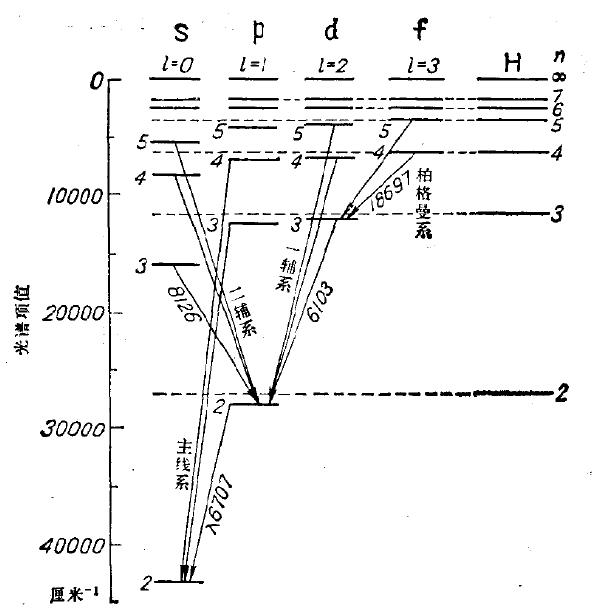
\includegraphics[width=0.4\linewidth]{figures/Energy-Level-Lithium}
  \caption{Energy Level of Lithium Atom}
  \label{fig:}
\end{figure}

The wavenumbers of spectroscopic lines

\begin{equation}
  \begin{aligned}
    \tilde{\nu}_n = \tilde{\nu}_{\infty} - \dfrac{R}{n^{*2}} 
  \end{aligned}
\end{equation}

\section{Self-spin and Orbital Angular Momentum}

\begin{equation*}
  \begin{aligned}
    s = \dfrac{1}{2} \quad l = 1,2,3,\dots \quad j = l \pm s
  \end{aligned}
\end{equation*}

\begin{table*}[h]
  \centering
  \begin{tabular}{|Sc|Sc|Sc|}
    \hline
    Self-spin & $p_s = \sqrt{s \left( s + 1 \right)} \hbar$ & $\mu_s = \dfrac{e}{m} p_s $ \\
    \hline
    Orbital & $p_l = \sqrt{l \left( l + 1 \right)} \hbar$ & $\mu_s = \dfrac{e}{2m} p_l $ \\
    \hline
    Total & $p_j = \sqrt{j \left( j + 1 \right)} \hbar$ & $\mu_j = g \dfrac{e}{2m} p_j $ \\
    \hline
  \end{tabular}
\end{table*}

\begin{equation*}
  \begin{aligned}
    \vec{p}_s + \vec{p}_l = \vec{p}_j
  \end{aligned}
\end{equation*}

\section{Selection Rule in Transition}

\begin{equation*}
  \left\{
    \begin{aligned}
      \Delta l &= \pm 1 \\
      \Delta j &= 0, \pm 1
    \end{aligned}
  \right.
\end{equation*}

%%% Local Variables:
%%% mode: latex
%%% TeX-master: "Atomic_Physics"
%%% End:
